\documentclass[aspectratio=169]{beamer}

\usepackage[utf8]{inputenc}
\usetheme{Singapore}
\usepackage{xcolor}
\setbeamertemplate{footline}[frame number]

\usepackage{amsmath,amssymb}

\usepackage{times}
\usepackage{ulem}

\usepackage{graphicx}
\usepackage{epstopdf}
\usepackage{tikz}

\setbeamercovered{dynamic}

% We add the following commonly used macros:

\usepackage{graphicx}
\graphicspath{{../imgs/}{imgs/}{./}}


% vectors as boldsymbols:
\newcommand{\bsa}{{\boldsymbol{a}}}
\newcommand{\bsb}{{\boldsymbol{b}}}
\newcommand{\bsc}{{\boldsymbol{c}}}
\newcommand{\bsd}{{\boldsymbol{d}}}
\newcommand{\bse}{{\boldsymbol{e}}}
\newcommand{\bsf}{{\boldsymbol{f}}}
\newcommand{\bsg}{{\boldsymbol{g}}}
\newcommand{\bsh}{{\boldsymbol{h}}}
\newcommand{\bsi}{{\boldsymbol{i}}}
\newcommand{\bsj}{{\boldsymbol{j}}}
\newcommand{\bsk}{{\boldsymbol{k}}}
\newcommand{\bsl}{{\boldsymbol{l}}}
\newcommand{\bsm}{{\boldsymbol{m}}}
\newcommand{\bsn}{{\boldsymbol{n}}}
\newcommand{\bso}{{\boldsymbol{o}}}
\newcommand{\bsp}{{\boldsymbol{p}}}
\newcommand{\bsq}{{\boldsymbol{q}}}
\newcommand{\bsr}{{\boldsymbol{r}}}
\newcommand{\bss}{{\boldsymbol{s}}}
\newcommand{\bst}{{\boldsymbol{t}}}
\newcommand{\bsu}{{\boldsymbol{u}}}
\newcommand{\bsv}{{\boldsymbol{v}}}
\newcommand{\bsw}{{\boldsymbol{w}}}
\newcommand{\bsx}{{\boldsymbol{x}}}
\newcommand{\bsy}{{\boldsymbol{y}}}
\newcommand{\bsz}{{\boldsymbol{z}}}
\newcommand{\bsA}{{\boldsymbol{A}}}
\newcommand{\bsB}{{\boldsymbol{B}}}
\newcommand{\bsC}{{\boldsymbol{C}}}
\newcommand{\bsD}{{\boldsymbol{D}}}
\newcommand{\bsE}{{\boldsymbol{E}}}
\newcommand{\bsF}{{\boldsymbol{F}}}
\newcommand{\bsG}{{\boldsymbol{G}}}
\newcommand{\bsH}{{\boldsymbol{H}}}
\newcommand{\bsI}{{\boldsymbol{I}}}
\newcommand{\bsJ}{{\boldsymbol{J}}}
\newcommand{\bsK}{{\boldsymbol{K}}}
\newcommand{\bsL}{{\boldsymbol{L}}}
\newcommand{\bsM}{{\boldsymbol{M}}}
\newcommand{\bsN}{{\boldsymbol{N}}}
\newcommand{\bsO}{{\boldsymbol{O}}}
\newcommand{\bsP}{{\boldsymbol{P}}}
\newcommand{\bsQ}{{\boldsymbol{Q}}}
\newcommand{\bsR}{{\boldsymbol{R}}}
\newcommand{\bsS}{{\boldsymbol{S}}}
\newcommand{\bsT}{{\boldsymbol{T}}}
\newcommand{\bsU}{{\boldsymbol{U}}}
\newcommand{\bsV}{{\boldsymbol{V}}}
\newcommand{\bsW}{{\boldsymbol{W}}}
\newcommand{\bsX}{{\boldsymbol{X}}}
\newcommand{\bsY}{{\boldsymbol{Y}}}
\newcommand{\bsZ}{{\boldsymbol{Z}}}
% other commonly used boldsymbols:
\newcommand{\bsell}{{\boldsymbol{\ell}}}
\newcommand{\bszero}{{\boldsymbol{0}}} % vector of zeros
\newcommand{\bsone}{{\boldsymbol{1}}}  % vector of ones
% boldsymbol greeks:
\newcommand{\bsalpha}{{\boldsymbol{\alpha}}}
\newcommand{\bsbeta}{{\boldsymbol{\beta}}}
\newcommand{\bsgamma}{{\boldsymbol{\gamma}}}
\newcommand{\bsdelta}{{\boldsymbol{\delta}}}
\newcommand{\bsepsilon}{{\boldsymbol{\epsilon}}}
\newcommand{\bsvarepsilon}{{\boldsymbol{\varepsilon}}}
\newcommand{\bszeta}{{\boldsymbol{\zeta}}}
\newcommand{\bseta}{{\boldsymbol{\eta}}}
\newcommand{\bstheta}{{\boldsymbol{\theta}}}
\newcommand{\bsvartheta}{{\boldsymbol{\vartheta}}}
\newcommand{\bskappa}{{\boldsymbol{\kappa}}}
\newcommand{\bslambda}{{\boldsymbol{\lambda}}}
\newcommand{\bsmu}{{\boldsymbol{\mu}}}
\newcommand{\bsnu}{{\boldsymbol{\nu}}}
\newcommand{\bsxi}{{\boldsymbol{\xi}}}
\newcommand{\bspi}{{\boldsymbol{\pi}}}
\newcommand{\bsvarpi}{{\boldsymbol{\varpi}}}
\newcommand{\bsrho}{{\boldsymbol{\rho}}}
\newcommand{\bsvarrho}{{\boldsymbol{\varrho}}}
\newcommand{\bssigma}{{\boldsymbol{\sigma}}}
\newcommand{\bsvarsigma}{{\boldsymbol{\varsigma}}}
\newcommand{\bstau}{{\boldsymbol{\tau}}}
\newcommand{\bsupsilon}{{\boldsymbol{\upsilon}}}
\newcommand{\bsphi}{{\boldsymbol{\phi}}}
\newcommand{\bsvarphi}{{\boldsymbol{\varphi}}}
\newcommand{\bschi}{{\boldsymbol{\chi}}}
\newcommand{\bspsi}{{\boldsymbol{\psi}}}
\newcommand{\bsomega}{{\boldsymbol{\omega}}}
\newcommand{\bsGamma}{{\boldsymbol{\Gamma}}}
\newcommand{\bsDelta}{{\boldsymbol{\Delta}}}
\newcommand{\bsTheta}{{\boldsymbol{\Theta}}}
\newcommand{\bsLambda}{{\boldsymbol{\Lambda}}}
\newcommand{\bsXi}{{\boldsymbol{\Xi}}}
\newcommand{\bsPi}{{\boldsymbol{\Pi}}}
\newcommand{\bsSigma}{{\boldsymbol{\Sigma}}}
\newcommand{\bsUpsilon}{{\boldsymbol{\Upsilon}}}
\newcommand{\bsPhi}{{\boldsymbol{\Phi}}}
\newcommand{\bsPsi}{{\boldsymbol{\Psi}}}
\newcommand{\bsOmega}{{\boldsymbol{\Omega}}}

% Roman fonts:
\newcommand{\rma}{{\mathrm{a}}}
\newcommand{\rmb}{{\mathrm{b}}}
\newcommand{\rmc}{{\mathrm{c}}}
\newcommand{\rmd}{{\mathrm{d}}}
\newcommand{\rme}{{\mathrm{e}}}
\newcommand{\rmf}{{\mathrm{f}}}
\newcommand{\rmg}{{\mathrm{g}}}
\newcommand{\rmh}{{\mathrm{h}}}
\newcommand{\rmi}{{\mathrm{i}}}
\newcommand{\rmj}{{\mathrm{j}}}
\newcommand{\rmk}{{\mathrm{k}}}
\newcommand{\rml}{{\mathrm{l}}}
\newcommand{\rmm}{{\mathrm{m}}}
\newcommand{\rmn}{{\mathrm{n}}}
\newcommand{\rmo}{{\mathrm{o}}}
\newcommand{\rmp}{{\mathrm{p}}}
\newcommand{\rmq}{{\mathrm{q}}}
\newcommand{\rmr}{{\mathrm{r}}}
\newcommand{\rms}{{\mathrm{s}}}
\newcommand{\rmt}{{\mathrm{t}}}
\newcommand{\rmu}{{\mathrm{u}}}
\newcommand{\rmv}{{\mathrm{v}}}
\newcommand{\rmw}{{\mathrm{w}}}
\newcommand{\rmx}{{\mathrm{x}}}
\newcommand{\rmy}{{\mathrm{y}}}
\newcommand{\rmz}{{\mathrm{z}}}
\newcommand{\rmA}{{\mathrm{A}}}
\newcommand{\rmB}{{\mathrm{B}}}
\newcommand{\rmC}{{\mathrm{C}}}
\newcommand{\rmD}{{\mathrm{D}}}
\newcommand{\rmE}{{\mathrm{E}}}
\newcommand{\rmF}{{\mathrm{F}}}
\newcommand{\rmG}{{\mathrm{G}}}
\newcommand{\rmH}{{\mathrm{H}}}
\newcommand{\rmI}{{\mathrm{I}}}
\newcommand{\rmJ}{{\mathrm{J}}}
\newcommand{\rmK}{{\mathrm{K}}}
\newcommand{\rmL}{{\mathrm{L}}}
\newcommand{\rmM}{{\mathrm{M}}}
\newcommand{\rmN}{{\mathrm{N}}}
\newcommand{\rmO}{{\mathrm{O}}}
\newcommand{\rmP}{{\mathrm{P}}}
\newcommand{\rmQ}{{\mathrm{Q}}}
\newcommand{\rmR}{{\mathrm{R}}}
\newcommand{\rmS}{{\mathrm{S}}}
\newcommand{\rmT}{{\mathrm{T}}}
\newcommand{\rmU}{{\mathrm{U}}}
\newcommand{\rmV}{{\mathrm{V}}}
\newcommand{\rmW}{{\mathrm{W}}}
\newcommand{\rmX}{{\mathrm{X}}}
\newcommand{\rmY}{{\mathrm{Y}}}
\newcommand{\rmZ}{{\mathrm{Z}}}
% also commonly defined
\newcommand{\rd}{{\mathrm{d}}}
\newcommand{\ri}{{\mathrm{i}}}

% blackboards:
\newcommand{\bbA}{{\mathbb{A}}}
\newcommand{\bbB}{{\mathbb{B}}}
\newcommand{\bbC}{{\mathbb{C}}}
\newcommand{\bbD}{{\mathbb{D}}}
\newcommand{\bbE}{{\mathbb{E}}}
\newcommand{\bbF}{{\mathbb{F}}}
\newcommand{\bbG}{{\mathbb{G}}}
\newcommand{\bbH}{{\mathbb{H}}}
\newcommand{\bbI}{{\mathbb{I}}}
\newcommand{\bbJ}{{\mathbb{J}}}
\newcommand{\bbK}{{\mathbb{K}}}
\newcommand{\bbL}{{\mathbb{L}}}
\newcommand{\bbM}{{\mathbb{M}}}
\newcommand{\bbN}{{\mathbb{N}}}
\newcommand{\bbO}{{\mathbb{O}}}
\newcommand{\bbP}{{\mathbb{P}}}
\newcommand{\bbQ}{{\mathbb{Q}}}
\newcommand{\bbR}{{\mathbb{R}}}
\newcommand{\bbS}{{\mathbb{S}}}
\newcommand{\bbT}{{\mathbb{T}}}
\newcommand{\bbU}{{\mathbb{U}}}
\newcommand{\bbV}{{\mathbb{V}}}
\newcommand{\bbW}{{\mathbb{W}}}
\newcommand{\bbX}{{\mathbb{X}}}
\newcommand{\bbY}{{\mathbb{Y}}}
\newcommand{\bbZ}{{\mathbb{Z}}}
% commonly used shortcuts:
\newcommand{\C}{{\mathbb{C}}} % complex numbers
\newcommand{\F}{{\mathbb{F}}} % field, finite field
\newcommand{\N}{{\mathbb{N}}} % natural numbers {1, 2, ...}
\newcommand{\Q}{{\mathbb{Q}}} % rationals
\newcommand{\R}{{\mathbb{R}}} % reals
\newcommand{\Z}{{\mathbb{Z}}} % integers
% more commonly used shortcuts:
\newcommand{\CC}{{\mathbb{C}}} % complex numbers
\newcommand{\FF}{{\mathbb{F}}} % field, finite field
\newcommand{\NN}{{\mathbb{N}}} % natural numbers {1, 2, ...}
\newcommand{\QQ}{{\mathbb{Q}}} % rationals
\newcommand{\RR}{{\mathbb{R}}} % reals
\newcommand{\ZZ}{{\mathbb{Z}}} % integers
% more commonly used shortcuts:
\newcommand{\EE}{{\mathbb{E}}}
\newcommand{\PP}{{\mathbb{P}}}
\newcommand{\TT}{{\mathbb{T}}}
\newcommand{\VV}{{\mathbb{V}}}
% and even more commonly used shortcuts:
\newcommand{\Complex}{{\mathbb{C}}}
\newcommand{\Integer}{{\mathbb{Z}}}
\newcommand{\Natural}{{\mathbb{N}}}
\newcommand{\Rational}{{\mathbb{Q}}}
\newcommand{\Real}{{\mathbb{R}}}

%%% Issue with miktex
% indicator boldface 1:
%\DeclareSymbolFont{bbold}{U}{bbold}{m}{n}
%\DeclareSymbolFontAlphabet{\mathbbold}{bbold}
%\newcommand{\ind}{{\mathbbold{1}}}
%\newcommand{\bbone}{{\mathbbold{1}}}


% calligraphic letters:
\newcommand{\cala}{{\mathcal{a}}}
\newcommand{\calb}{{\mathcal{b}}}
\newcommand{\calc}{{\mathcal{c}}}
\newcommand{\cald}{{\mathcal{d}}}
\newcommand{\cale}{{\mathcal{e}}}
\newcommand{\calf}{{\mathcal{f}}}
\newcommand{\calg}{{\mathcal{g}}}
\newcommand{\calh}{{\mathcal{h}}}
\newcommand{\cali}{{\mathcal{i}}}
\newcommand{\calj}{{\mathcal{j}}}
\newcommand{\calk}{{\mathcal{k}}}
\newcommand{\call}{{\mathcal{l}}}
\newcommand{\calm}{{\mathcal{m}}}
\newcommand{\caln}{{\mathcal{n}}}
\newcommand{\calo}{{\mathcal{o}}}
\newcommand{\calp}{{\mathcal{p}}}
\newcommand{\calq}{{\mathcal{q}}}
\newcommand{\calr}{{\mathcal{r}}}
\newcommand{\cals}{{\mathcal{s}}}
\newcommand{\calt}{{\mathcal{t}}}
\newcommand{\calu}{{\mathcal{u}}}
\newcommand{\calv}{{\mathcal{v}}}
\newcommand{\calw}{{\mathcal{w}}}
\newcommand{\calx}{{\mathcal{x}}}
\newcommand{\caly}{{\mathcal{y}}}
\newcommand{\calz}{{\mathcal{z}}}
\newcommand{\calA}{{\mathcal{A}}}
\newcommand{\calB}{{\mathcal{B}}}
\newcommand{\calC}{{\mathcal{C}}}
\newcommand{\calD}{{\mathcal{D}}}
\newcommand{\calE}{{\mathcal{E}}}
\newcommand{\calF}{{\mathcal{F}}}
\newcommand{\calG}{{\mathcal{G}}}
\newcommand{\calH}{{\mathcal{H}}}
\newcommand{\calI}{{\mathcal{I}}}
\newcommand{\calJ}{{\mathcal{J}}}
\newcommand{\calK}{{\mathcal{K}}}
\newcommand{\calL}{{\mathcal{L}}}
\newcommand{\calM}{{\mathcal{M}}}
\newcommand{\calN}{{\mathcal{N}}}
\newcommand{\calO}{{\mathcal{O}}}
\newcommand{\calP}{{\mathcal{P}}}
\newcommand{\calQ}{{\mathcal{Q}}}
\newcommand{\calR}{{\mathcal{R}}}
\newcommand{\calS}{{\mathcal{S}}}
\newcommand{\calT}{{\mathcal{T}}}
\newcommand{\calU}{{\mathcal{U}}}
\newcommand{\calV}{{\mathcal{V}}}
\newcommand{\calW}{{\mathcal{W}}}
\newcommand{\calX}{{\mathcal{X}}}
\newcommand{\calY}{{\mathcal{Y}}}
\newcommand{\calZ}{{\mathcal{Z}}}

% Euler fraks:
\newcommand{\fraka}{{\mathfrak{a}}}
\newcommand{\frakb}{{\mathfrak{b}}}
\newcommand{\frakc}{{\mathfrak{c}}}
\newcommand{\frakd}{{\mathfrak{d}}}
\newcommand{\frake}{{\mathfrak{e}}}
\newcommand{\frakf}{{\mathfrak{f}}}
\newcommand{\frakg}{{\mathfrak{g}}}
\newcommand{\frakh}{{\mathfrak{h}}}
\newcommand{\fraki}{{\mathfrak{i}}}
\newcommand{\frakj}{{\mathfrak{j}}}
\newcommand{\frakk}{{\mathfrak{k}}}
\newcommand{\frakl}{{\mathfrak{l}}}
\newcommand{\frakm}{{\mathfrak{m}}}
\newcommand{\frakn}{{\mathfrak{n}}}
\newcommand{\frako}{{\mathfrak{o}}}
\newcommand{\frakp}{{\mathfrak{p}}}
\newcommand{\frakq}{{\mathfrak{q}}}
\newcommand{\frakr}{{\mathfrak{r}}}
\newcommand{\fraks}{{\mathfrak{s}}}
\newcommand{\frakt}{{\mathfrak{t}}}
\newcommand{\fraku}{{\mathfrak{u}}}
\newcommand{\frakv}{{\mathfrak{v}}}
\newcommand{\frakw}{{\mathfrak{w}}}
\newcommand{\frakx}{{\mathfrak{x}}}
\newcommand{\fraky}{{\mathfrak{y}}}
\newcommand{\frakz}{{\mathfrak{z}}}
\newcommand{\frakA}{{\mathfrak{A}}}
\newcommand{\frakB}{{\mathfrak{B}}}
\newcommand{\frakC}{{\mathfrak{C}}}
\newcommand{\frakD}{{\mathfrak{D}}}
\newcommand{\frakE}{{\mathfrak{E}}}
\newcommand{\frakF}{{\mathfrak{F}}}
\newcommand{\frakG}{{\mathfrak{G}}}
\newcommand{\frakH}{{\mathfrak{H}}}
\newcommand{\frakI}{{\mathfrak{I}}}
\newcommand{\frakJ}{{\mathfrak{J}}}
\newcommand{\frakK}{{\mathfrak{K}}}
\newcommand{\frakL}{{\mathfrak{L}}}
\newcommand{\frakM}{{\mathfrak{M}}}
\newcommand{\frakN}{{\mathfrak{N}}}
\newcommand{\frakO}{{\mathfrak{O}}}
\newcommand{\frakP}{{\mathfrak{P}}}
\newcommand{\frakQ}{{\mathfrak{Q}}}
\newcommand{\frakR}{{\mathfrak{R}}}
\newcommand{\frakS}{{\mathfrak{S}}}
\newcommand{\frakT}{{\mathfrak{T}}}
\newcommand{\frakU}{{\mathfrak{U}}}
\newcommand{\frakV}{{\mathfrak{V}}}
\newcommand{\frakW}{{\mathfrak{W}}}
\newcommand{\frakX}{{\mathfrak{X}}}
\newcommand{\frakY}{{\mathfrak{Y}}}
\newcommand{\frakZ}{{\mathfrak{Z}}}
% sets as Euler fraks:
\newcommand{\seta}{{\mathfrak{a}}}
\newcommand{\setb}{{\mathfrak{b}}}
\newcommand{\setc}{{\mathfrak{c}}}
\newcommand{\setd}{{\mathfrak{d}}}
\newcommand{\sete}{{\mathfrak{e}}}
\newcommand{\setf}{{\mathfrak{f}}}
\newcommand{\setg}{{\mathfrak{g}}}
\newcommand{\seth}{{\mathfrak{h}}}
\newcommand{\seti}{{\mathfrak{i}}}
\newcommand{\setj}{{\mathfrak{j}}}
\newcommand{\setk}{{\mathfrak{k}}}
\newcommand{\setl}{{\mathfrak{l}}}
\newcommand{\setm}{{\mathfrak{m}}}
\newcommand{\setn}{{\mathfrak{n}}}
\newcommand{\seto}{{\mathfrak{o}}}
\newcommand{\setp}{{\mathfrak{p}}}
\newcommand{\setq}{{\mathfrak{q}}}
\newcommand{\setr}{{\mathfrak{r}}}
\newcommand{\sets}{{\mathfrak{s}}}
\newcommand{\sett}{{\mathfrak{t}}}
\newcommand{\setu}{{\mathfrak{u}}}
\newcommand{\setv}{{\mathfrak{v}}}
\newcommand{\setw}{{\mathfrak{w}}}
\newcommand{\setx}{{\mathfrak{x}}}
\newcommand{\sety}{{\mathfrak{y}}}
\newcommand{\setz}{{\mathfrak{z}}}
\newcommand{\setA}{{\mathfrak{A}}}
\newcommand{\setB}{{\mathfrak{B}}}
\newcommand{\setC}{{\mathfrak{C}}}
\newcommand{\setD}{{\mathfrak{D}}}
\newcommand{\setE}{{\mathfrak{E}}}
\newcommand{\setF}{{\mathfrak{F}}}
\newcommand{\setG}{{\mathfrak{G}}}
\newcommand{\setH}{{\mathfrak{H}}}
\newcommand{\setI}{{\mathfrak{I}}}
\newcommand{\setJ}{{\mathfrak{J}}}
\newcommand{\setK}{{\mathfrak{K}}}
\newcommand{\setL}{{\mathfrak{L}}}
\newcommand{\setM}{{\mathfrak{M}}}
\newcommand{\setN}{{\mathfrak{N}}}
\newcommand{\setO}{{\mathfrak{O}}}
\newcommand{\setP}{{\mathfrak{P}}}
\newcommand{\setQ}{{\mathfrak{Q}}}
\newcommand{\setR}{{\mathfrak{R}}}
\newcommand{\setS}{{\mathfrak{S}}}
\newcommand{\setT}{{\mathfrak{T}}}
\newcommand{\setU}{{\mathfrak{U}}}
\newcommand{\setV}{{\mathfrak{V}}}
\newcommand{\setW}{{\mathfrak{W}}}
\newcommand{\setX}{{\mathfrak{X}}}
\newcommand{\setY}{{\mathfrak{Y}}}
\newcommand{\setZ}{{\mathfrak{Z}}}

% other commonly defined commands:
\newcommand{\wal}{{\rm wal}}
\newcommand{\floor}[1]{\left\lfloor #1 \right\rfloor} % floor
\newcommand{\ceil}[1]{\left\lceil #1 \right\rceil}    % ceil
\DeclareMathOperator{\cov}{Cov}
\DeclareMathOperator{\var}{Var}
\providecommand{\argmin}{\operatorname*{argmin}}
\providecommand{\argmax}{\operatorname*{argmax}}

% Colour switches inherited from PSTricks ({\red ...}, {\blue ...}).
% Defined here so that decks no longer need to load pstricks just for them.
\providecommand{\red}{\color{red}}
\providecommand{\blue}{\color{blue}}


\def\bxi{\boldsymbol\xi}
\def\bepsilon{\boldsymbol\epsilon}
\def\bomega{\boldsymbol\omega}
\def\aff{\operatorname{aff}}
\def\cR{\mathcal{R}}

\newcommand{\tim}[1]{\;\; \mbox{#1} \;\;}

\title[Chance-constrained programming]{Stochastic optimization\\Chance-constrained programming}

\author[Fabian Bastin]{Fabian Bastin \\ \texorpdfstring{\url{fabian.bastin@umontreal.ca}}{fabian.bastin@umontreal.ca} \\ Université de Montréal -- CIRRELT -- IVADO}

\date{}

\begin{document}

%% AJOUTER DISCUSSION BIRGE ET LOUVEAUX P128

\frame{\titlepage}

\begin{frame}
\frametitle{A long story}

\begin{itemize}
	\item 
Introduced in 1959 by Charnes and Cooper \url{https://dl.acm.org/doi/10.1287/mnsc.6.1.73}
	\item 
And also a bit improbable.
	\item 
Cooper dropped out of high school to support his family, and became a professional boxer.
	\item 
He became an accountant for Eric Louis Kohler, whom he met while hitchhiking.
	\item 
Kohler financed his bachelor's degree at the University of Chicago.
\item
At 26, he enrolled at Columbia University and finished his coursework and dissertation, but never received his PhD due to his dissertation's claim that decision making was not a centralized process.
\end{itemize}

\end{frame}
\begin{frame}
\frametitle{A long story (cont'd)}
	
\begin{itemize}
\item
The collaboration with Charnes was however successful, with more than 200 publications, and led to a successful academic career.
\item 
Source: \url{https://www.informs.org/Explore/History-of-O.R.-Excellence/Biographical-Profiles/Cooper-William-W}
\end{itemize}

\end{frame}

\begin{frame}[fragile]
\frametitle{Cooper and Charnes}

\begin{center}

\includegraphics[width=0.4\textwidth,height=0.62\textheight,keepaspectratio]{coopercharnes.png}

John von Neumann Theory Prize, 1982 (with Richard J. Duffin)
\end{center}

\end{frame}

\begin{frame}
\frametitle{Mathematical Formulation}

$$
\begin{aligned}
	\min_{x \in \calX} \quad & \EE[f(x, \xi)] \\
	\text{s.t.} \quad & P[ g_i(x, \xi) \leq 0 ] \geq 1 - \alpha_i, \quad i = 1, \ldots, m,
\end{aligned}
$$
where:
\begin{itemize}
	\item \( \xi \in \RR^p \) is a random vector with known probability distribution \( P \);
	\item \( x \in \RR^n \) is the vector of decision variables;
	\item \( \calX \subseteq \RR^n \) is a convex deterministic set;
	\item \( f(x, \xi) \) is the cost function;
	\item \( g_i(x, \xi) \) are random constraint functions;
	\item \( \alpha_i \in (0, 1) \) specifies the acceptable risk level for constraint \( i \).
\end{itemize}

\end{frame}

\begin{frame}
\frametitle{Probabilistic constraints}

The probabilistic constraint 
\[
P[ g_i(x, \xi) \leq 0 ] \geq 1 - \alpha_i
\]
ensures that constraint \( i \) is satisfied with probability at least \( 1 - \alpha_i \). Equivalently, the probability of violation 
\[
P[ g_i(x, \xi) > 0 ] \leq \alpha_i
\]
is limited to a user-specified tolerance. Smaller values of \( \alpha_i \) produce more conservative, risk-averse solutions.

\end{frame}

\begin{frame}
\frametitle{Individual and joint chance constraints}

Two common variants are:
\begin{enumerate}
	\item \textbf{Individual (or separate) chance constraints:} each constraint \( g_i(x, \xi) \leq 0 \) is required to hold with probability at least \( 1 - \alpha_i \);
	\item \textbf{Joint chance constraints:}
	\[
	P[ g_i(x, \xi) \leq 0, \, i=1,\ldots,m ] \geq 1 - \alpha,
	\]
	which ensures simultaneous satisfaction of all constraints with a single confidence level \( 1 - \alpha \).
\end{enumerate}
%The joint form is more conservative and significantly harder to handle computationally.

\end{frame}

\begin{frame}
\frametitle{Toy example}

Source: J. Linderoth (\url{https://jlinderoth.github.io/classes/ie495/lecture22.pdf})

\mbox{}

Consider the toy problem
\begin{align*}
\min_x\ & x_1 + x_2 \\
\text{s.t. } & \xi_1 x_1 + x_2 \geq 7 \\
& \xi_2 x_1 + x_2 \geq 4 \\
& x_1, x_2 \geq 0.
\end{align*}

\mbox{} 

Instead of requiring that a constraint holds for all the scenarios, we can require that the constraint is satisfied with a given (large) probability.

\end{frame}

\begin{frame}
\frametitle{Chance constraints}

\begin{enumerate}
\item 
Separate chance constraints
\begin{align*}
P [ \xi_1x_1 + x_2 \geq 7 ] &\geq 1-\alpha_1 \\
P [ \xi_2x_1 + x_2 \geq 4 ] &\geq 1-\alpha_2
\end{align*}
\item
Joint chance constraint
\[
P [ \xi_1x_1 + x_2 \geq 7, \; \xi_2x_1 + x_2 \geq 4 ] \geq 1-\alpha
\]
\end{enumerate}

\end{frame}

\begin{frame}
\frametitle{Example: joint chance constraints}

\begin{align}
P[(\xi_1, \xi_2) = (1,1)] &= 0.1 \label{eq:scen1} \\
P[(\xi_1, \xi_2) = (2,5/9)] &= 0.4 \label{eq:scen2} \\
P[(\xi_1, \xi_2) = (3,7/9)] &= 0.4 \label{eq:scen3} \\
P[(\xi_1, \xi_2) = (4,1/3)] &= 0.1 \label{eq:scen4}
\end{align}

\mbox{}

Assume that $\alpha \in [0.1,0.2)$, and we have the joint constraint
\[
P [ \xi_1x_1 + x_2 \geq 7, \; \xi_2x_1 + x_2 \geq 4 ] \geq 1-\alpha
\]

\mbox{}

We then have to satisfy the constraints in scenarios \eqref{eq:scen2} and \eqref{eq:scen3}, and in either \eqref{eq:scen1} or \eqref{eq:scen4}.

\end{frame}

\begin{frame}
\frametitle{Example: frontiers of constraints}

\begin{center}
\includegraphics<1>[width=\textwidth,height=0.75\textheight,keepaspectratio]{"chance_constraint_feasible_region.pdf"}
\end{center}

\end{frame}

\begin{frame}
\frametitle{Feasible set}

Feasible set:
\[
K_1(\alpha) = \lbrace x \,|\, P[g_i(x,\bxi) \leq 0] \geq 1-\alpha_i,\ i=1,\ldots,m \rbrace
\]

\mbox{}

$K_1(\alpha)$ is not necessarily convex, even if $g_i(x,\bxi)$, $i=1,\ldots,m$, are linear in $x$: the joint constraint of the example yields a union of two polyhedra.

\end{frame}

\begin{frame}
\frametitle{Quasi-concavity}

\begin{definition}[Quasi-Concavity]
	A function $f: S \to \mathbb{R}$, where $S \subseteq \mathbb{R}^n$ is a convex set, is \textbf{quasi-concave} if for all $\bsx, \bsy \in S$ and all $\lambda \in [0,1]$:
	\[
	f(\lambda\bsx + (1-\lambda)\bsy) \geq \min\{f(\bsx), f(\bsy)\}
	\]
\end{definition}

\begin{definition}
The probability measure $P$ defined on the Borel sets of $\RR^n$ is
said to be quasi-concave, if for any convex subsets $A$, $B$ of $\RR^n$,
and any $\lambda \in [0,1]$,
\[
P[(1-\lambda)A+\lambda B] \geq \min \lbrace P[A], P[B] \rbrace.
\]
\end{definition}

(See Prékopa (2003), ``Probabilistic Programming'', Chapter 5 in ``\href{https://www.sciencedirect.com/handbook/handbooks-in-operations-research-and-management-science/vol/10}{Stochastic Programming}'')

\end{frame}

\begin{frame}
\frametitle{Applications in optimization}

\begin{theorem}[Convexity of Upper Level Sets]
	Let $f: S \to \RR$ be a quasi-concave function, where $S \subseteq \RR^n$ is a convex set. Then for any $t \in \RR$, the upper level set
	\[
	U_t = \{\bsx \in S \mid f(\bsx) \geq t\}
	\]
	is convex.
\end{theorem}

\begin{corollary}[Feasible Set Convexity]
	If $f$ is quasi-concave, then the constraint:
	\[
	f(\bsx) \geq t
	\]
	defines a \textbf{convex feasible set} for any $t \in \mathbb{R}$.
\end{corollary}

\end{frame}

\begin{frame}
\frametitle{Applications in stochastic programming}

For chance-constrained programming problems of the form:
\[
P[g(\bsx,\bsxi) \leq 0] \geq 1-\alpha,
\]
if $P[g(\bsx,\bsxi)\leq 0]$ is quasi-concave in $\bsx$, 
then $\{ \bsx \mid P[g(\bsx,\bsxi) \leq 0] \geq 1-\alpha\}$ is \textbf{convex}: with a convex objective, the problem is a convex program.

\smallskip

Convexity is not tractability, though: evaluating the probability and its gradient still requires multivariate integration.

\end{frame}

\begin{frame}
\frametitle{Log-concavity}

\begin{definition}[Log-Concave Function]
	A function $f: S \to \mathbb{R}_+$, where $S \subseteq \mathbb{R}^n$ is a convex set, is \textbf{log-concave} if for all $\bsx, \bsy \in S$ and $\lambda \in [0,1]$:
	\[
	f(\lambda \bsx + (1-\lambda)\bsy) \geq f(\bsx)^\lambda \, f(\bsy)^{1-\lambda}
	\]
\end{definition}

A log-concave function is quasi-concave, as $f(\bsx)^\lambda \, f(\bsy)^{1-\lambda} \geq \min\{f(\bsx), f(\bsy)\}$.

\smallskip

A probability measure $P$ is \textbf{log-concave} if $P[\lambda A + (1-\lambda) B] \geq P[A]^{\lambda} P[B]^{1-\lambda}$ for all convex sets $A$, $B$ and $\lambda \in [0,1]$; this holds as soon as $P$ has a log-concave density (Prékopa, 1973).

\end{frame}

\begin{frame}
	\frametitle{Jointly Convex Constraint Function}

\begin{definition}
	A constraint function $g: \RR^n \times \RR^p \to \RR$ is \textbf{jointly convex} in $(\bsx, \bsxi)$ if for all $(\bsx_1, \bsxi_1), (\bsx_2, \bsxi_2) \in \RR^n \times \RR^p$ and all $\lambda \in [0,1]$:
	\[
	g(\lambda \bsx_1 + (1-\lambda)\bsx_2, \lambda \bsxi_1 + (1-\lambda)\bsxi_2) \leq \lambda g(\bsx_1, \bsxi_1) + (1-\lambda) g(\bsx_2, \bsxi_2)
	\]
\end{definition}

\end{frame}

\begin{frame}
\frametitle{Prékopa's fundamental theorem}

\begin{theorem}
Let $\bsxi \in \RR^p$ be a random vector with log-concave probability distribution, and let $g: \RR^n \times \RR^p \to \RR$ be jointly quasi-convex in $(\bsx, \bsxi)$. Then the probability function
\[
	\phi(\bsx) = P[ g(\bsx, \bsxi) \leq 0 ]
\]
is log-concave (and hence quasi-concave) in $\bsx$.
\end{theorem}

\mbox{}

(Prékopa, A. (1973). On logarithmic concave measures and functions.
Acta Scientiarum Mathematicarum 34, 335--343)
\end{frame}

\begin{frame}
\frametitle{Examples of jointly quasi-convex functions}

\begin{example}[Affine in $(\bsx, \bsxi)$]
	If $g(\bsx, \bsxi) = \mathbf{a}^\top \bsx + \mathbf{b}^\top \bsxi + c$, where $\mathbf{a} \in \mathbb{R}^n$, $\mathbf{b} \in \mathbb{R}^p$, $c \in \mathbb{R}$, then $g$ is jointly quasi-convex (in fact, jointly convex).
\end{example}

\begin{example}[Maximum]
The maximum of quasi-convex functions is quasi-convex.
\end{example}

\end{frame}

\begin{frame}
\frametitle{Common log-concave distributions}

{\small
\begin{align*}
	\text{Normal:} &\quad f(x) = \frac{1}{\sqrt{2\pi\sigma^2}} \exp\left(-\frac{(x-\mu)^2}{2\sigma^2}\right) \\
	\text{Exponential:} &\quad f(x) = \lambda \exp(-\lambda x), \quad x \geq 0 \\
	\text{Uniform on convex } S: &\quad f(x) = \frac{1}{\operatorname{vol}(S)}, \quad x \in S \\
	\text{Gamma (shape $k \geq 1$):} &\quad f(x) = \frac{\lambda^k}{\Gamma(k)} x^{k-1} e^{-\lambda x}, \quad x > 0, \; \lambda > 0 \\
	\text{Beta ($a \geq 1, b \geq 1$):} &\quad f(x) = \frac{x^{a-1}(1-x)^{b-1}}{B(a,b)}, \quad x \in [0,1]\\
	\text{Multivariate normal:} &\quad f(x) = \frac{1}{\sqrt{(2\pi)^n \det(\Sigma)}} \exp\left( -\frac{1}{2}(x-\mu)^T \Sigma^{-1} (x-\mu) \right)
\end{align*}
}

\end{frame}

\begin{frame}
\frametitle{Solution methods for log-concave distributions}

With such a distribution, the feasible set is convex, and you can
\begin{itemize}
\item
use Lagrangian techniques
\item
use a reduced-gradient technique (see Kall \& Wallace, Section~4.1)
\end{itemize}

\end{frame}

\begin{frame}
\frametitle{Joint constraints}

\begin{theorem}[Prékopa's Theorem for Joint Constraints]
	If
	\begin{enumerate}
		\item $\bsxi$ has a log-concave probability distribution, and
		\item the set $\{(\bsx, \bsxi) \mid g_i(\bsx, \bsxi) \leq 0, \ i=1,\dots,m\}$ is convex, for instance because each $g_i$ is jointly quasi-convex in $(\bsx, \bsxi)$,
	\end{enumerate}
	then the function
	\[
	\phi(\bsx) = P\left[ g_i(\bsx, \bsxi) \leq 0, \ i=1,\dots,m \right]
	\]
	is log-concave (hence quasi-concave) in $\bsx$, and thus the feasible set $\{\bsx \mid \phi(\bsx) \geq 1-\alpha\}$ is convex.
\end{theorem}

\end{frame}

\begin{frame}
\frametitle{Maximum reformulation}

For joint constraints $P[g_j(\bsx, \bsxi) \leq 0,\ j=1,\ldots,m] \geq 1-\alpha$, define:
\[
G(\bsx, \bsxi) = \max_{j=1,\dots,m} g_j(\bsx, \bsxi)
\]
Then the constraint becomes:
\[
P[ G(\bsx, \bsxi) \leq 0 ] \geq 1-\alpha
\]
If every $g_j$ is jointly quasi-convex, so is $G$: Prékopa's theorem for a single constraint then covers joint constraints.

\end{frame}

\begin{frame}
\frametitle{Further reading}

For a more complete analysis of convexity in chance-constrained programming, see Section~4.2 in \href{https://epubs.siam.org/doi/book/10.1137/1.9781611976595}{Lectures on Stochastic Programming: Modeling and Theory} (3rd edition, Shapiro, Dentcheva, Ruszczy\'nski).

\end{frame}

\begin{frame}
	\frametitle{Linear inequalities}
	
Assume that the chance constraint can be written in the form
	$$
	P[T(\bxi)x \geq h(\bxi)] \geq 1-\alpha.
	$$
	
	\begin{theorem}
		Suppose $T(\bxi) = T$ is fixed, and $h(\bxi)$ has a quasi-concave
		probability measure $P$. Then $K_1(\alpha)$ is convex for $0 \leq \alpha \leq 1$.
	\end{theorem}
	
\end{frame}

\begin{frame}
\frametitle{Single constraint: easy case}

\begin{itemize}
	\item 
The situation in the single constraint case is sometimes simple.
\item 
Suppose again that $T_i (\bxi) = T_i$ is constant. Then
\[
P[T_i x \geq h_i (\bxi)] = F_{h_i}(T_i x) \geq 1-\alpha
\]
so the deterministic equivalent is
\[
T_i x \geq F_{h_i}^{-1}(1-\alpha)
\]
\ldots linear constraint! The resulting problem is still linear: compared with requiring $T_i x \geq h_i(\xi)$ for every realization, the worst case of $h_i(\bxi)$ is replaced by its $(1-\alpha)$-quantile.
\item
Recall that the inverse of the cdf is defined as
\[
F_{h_i}^{-1}(p) = \inf \lbrace t : F_{h_i} (t)  \geq p \rbrace, \quad p \in (0,1).
\]
\end{itemize}

\end{frame}

\begin{frame}
\frametitle{Other ``solvable'' cases}

Consider a single constraint $\bxi^T x \geq h$, with $h \in \RR$ fixed and $\bxi = (\xi_1, \xi_2,\ldots, \xi_n)$ following a multivariate normal distribution with mean $\mu$ and positive definite covariance matrix $\Sigma$.
Then, for $x \neq 0$,
\[
\frac{\sum_{i = 1}^n \xi_i x_i - \mu^T x}{\sqrt{x^T\Sigma x}} \sim N(0,1),
\]
and
\[
K_1(\alpha) = \lbrace x \mid \mu^T x \geq h + \Phi^{-1}(1-\alpha) \sqrt{x^T\Sigma x} \rbrace,
\]
where $\Phi$ is the standard normal cdf.

\smallskip

$K_1(\alpha)$ is a convex set for $\alpha \leq 0.5$. For $\alpha < 0.5$, it can be expressed as a second-order cone constraint:
\[
\| \Sigma^{1/2} x \|_2 \leq \frac{1}{\Phi^{-1}(1-\alpha)} (\mu^T x - h)
\]

\end{frame}

\begin{frame}
\frametitle{Second-order cone programming}

A second-order cone program (SOCP) is a convex optimization problem of the form
\begin{align*}
\min_x \ & f^T x \\
\text{s.t. } &
\| A_i x + b_i \|_2 \leq c_i^T x + d_i,\ i = 1,\ldots,m \\
& F x = g
\end{align*}
where $x \in \RR^n$, $f, c_i \in \RR^n$, $A_i \in \RR^{n_i \times n}$, $b_i \in \RR^{n_i}$, $d_i \in \RR$, $F \in \RR^{p \times n}$, and $g \in \RR^p$.

\smallskip

SOCPs can be solved efficiently by interior point methods.

\end{frame}

\begin{frame}
\frametitle{Example: chance-constrained portfolio optimization}

(Taken from S. Boyd and J. Linderoth)

\begin{itemize}
	\item 
Suppose we want to invest in $n$ assets, providing random return rates $\beta_1, \beta_2,\ldots, \beta_n$.
\item
$\bsbeta \sim N(\bsmu, \Sigma)$.
\item
$W$: total budget to invest.
\item
Suppose that we want to ensure a return of at least $b$.
We cannot guarantee it all the time, but we want it to occur most of the time.
\end{itemize}

\end{frame}

\begin{frame}
\frametitle{Example: chance-constrained portfolio optimization (cont'd)}

Let $x_i \geq 0$ be the amount invested in asset $i$.
Constraints:
\begin{align}
& P\left[ \sum_{i = 1}^n \beta_i x_i \geq b  \right] \geq 1-\alpha \label{eq:var_constraint} \\
& \sum_{i = 1}^n x_i \leq W \nonumber \\
& x_i \geq 0,\ i = 1,\ldots,n.  \nonumber
\end{align}

\smallskip

If $b < 0$, \eqref{eq:var_constraint} bounds the loss $-\beta^Tx$ by $-b$ with probability at least $1-\alpha$: a \textcolor{red}{Value-at-Risk constraint} (Ruszczyński and Shapiro, 2003).

\end{frame}

\begin{frame}
\frametitle{Example: deterministic equivalent of the chance constraint}

The return $\beta^T x$ is normal, with mean $\mu^T x$ and variance $x^T \Sigma x$.
For $x \neq 0$ and $\Sigma$ positive definite,
\[
Z = \frac{\beta^T x - \mu^T x}{\sqrt{x^T\Sigma x}} \sim N(0,1).
\]
Standardizing, then using the symmetry of $N(0,1)$, $1 - \Phi(-t) = \Phi(t)$:
\[
P\left[ \beta^T x \geq b \right]
= P\left[ Z \geq \frac{b - \mu^T x}{\sqrt{x^T\Sigma x}} \right]
= 1 - \Phi\left( \frac{b - \mu^T x}{\sqrt{x^T\Sigma x}} \right)
= \Phi\left( \frac{\mu^T x - b}{\sqrt{x^T\Sigma x}} \right).
\]
As $\Phi$ is continuous and increasing, \eqref{eq:var_constraint} holds if and only if
\[
\frac{\mu^T x - b}{\sqrt{x^T\Sigma x}} \geq \Phi^{-1}(1-\alpha)
\quad \Longleftrightarrow \quad
\mu^Tx - \Phi^{-1}(1-\alpha) \sqrt{x^T\Sigma x} \geq b.
\]
For $\alpha < 0.5$, $\Phi^{-1}(1-\alpha) > 0$, and this is a {\red second-order cone constraint}.

\end{frame}

\begin{frame}
\frametitle{Example: chance-constrained portfolio optimization (cont'd)}

We can also interpret $x_i$ as the proportion of the portfolio invested in asset $i$, by normalizing $\sum_{i=1}^n x_i = 1$.
Here $b$ is the minimum return rate of the portfolio and $x$ is the portfolio allocation vector.

\smallskip

We can add constraints on $x$ to ensure diversification, summarized by requiring $x \in \mathcal{C}$.

\smallskip

A complete program can now be expressed as:
\begin{align*}
\max_x \ & \EE[\beta^T x] = \mu^T x \\
\text{s.t. } & P\left[ \beta^T x \geq b \right] \geq 1-\alpha  \\
& \sum_{i = 1}^n x_i = 1 \\
& x \in \calC
\end{align*}

\end{frame}

\begin{frame}
\frametitle{Example: loss constraint}

Setting $b$ to 0 means that we want to ensure that we will not suffer a loss with high probability. Typically, $\alpha$ is set to 0.1, 0.05, 0.01,\ldots

\smallskip

As $\beta^T x$ has a continuous distribution, the chance constraint can also be expressed as
\[
P\left[ \beta^T x \leq 0 \right] \leq \alpha.
\]

\smallskip

We can also allow short selling by permitting some $x_i$ to be negative.
\end{frame}

\begin{frame}
\frametitle{Numerical illustration}

(Taken from S. Boyd -- \url{http://ee364a.stanford.edu/lectures/chance_constr.pdf})

$n = 10$ assets, $\alpha = 0.05$,$\mathcal{C} = \{x \mid x \succeq -0.1\}$

\smallskip

Compare:
\begin{itemize}
\item
optimal portfolio
\item
optimal portfolio without loss risk constraint
\item
uniform portfolio $(1/n)\mathbf{1}$
\end{itemize}

\begin{center}
\begin{tabular}{c|c|c}
portfolio & $\EE[\beta^T x]$ & $P[\beta^T x \leq 0]$ \\
\hline
optimal & 7.51 & 5.0\% \\
w/o loss constraint & 10.66 & 20.3\% \\
uniform & 3.41 & 18.9\%
\end{tabular}
\end{center}

\end{frame}

% Analytical solution if the non-negativity constraints are removed.
% See page 10 https://www.sciencedirect.com/science/article/pii/S0927050703100011

\begin{frame}
\frametitle{Short selling case}

Let's ignore the non-negativity and budget constraints and consider the program (Ruszczyński and Shapiro, 2003)
\begin{align*}
	\min_x \ & -\mu^T x \\
	\text{s.t. } & z_{\alpha} \sqrt{x^T\Sigma x} - \mu^Tx + b \leq 0,
\end{align*}
with $z_{\alpha} = \Phi^{-1}(1-\alpha) > 0$, i.e., $\alpha < 0.5$.

The Lagrangian is
\begin{align*}
L(x, \lambda) &= -\mu^T x + \lambda \left( z_{\alpha} \sqrt{x^T\Sigma x} - \mu^Tx + b \right) \\
&= -(1+\lambda) \mu^T x + \lambda z_{\alpha} \sqrt{x^T\Sigma x} + \lambda b
\end{align*}

\end{frame}

\begin{frame}
\frametitle{Reminder: KKT conditions}

For $\min_x f(x)$ s.t. $g(x) \leq 0$, with $f$ and $g$ continuously differentiable and $L(x,\lambda) = f(x) + \lambda g(x)$, the Karush-Kuhn-Tucker (KKT) conditions are
\begin{align*}
\nabla_x L(x,\lambda) &= 0 & \text{(stationarity)} \\
g(x) &\leq 0 & \text{(primal feasibility)} \\
\lambda g(x) &= 0 & \text{(complementarity)} \\
\lambda &\geq 0 & \text{(dual feasibility)}
\end{align*}
\begin{itemize}
\item
{\red Necessary}: a local minimizer satisfies them, for some $\lambda$, under a constraint qualification. For a convex problem, the Slater condition suffices: $g(\bar{x}) < 0$ for some $\bar{x}$.
\item
{\red Sufficient} for a convex problem: a KKT point is a global minimizer.
\end{itemize}

\smallskip

{\footnotesize (See the KKT background notes.)}

\end{frame}

\begin{frame}
	\frametitle{Short selling case: KKT conditions}

\begin{align*}
&	\nabla_x L(x, \lambda) = 0, && \lambda \geq 0, \\
&	z_{\alpha} \sqrt{x^T\Sigma x} - \mu^Tx + b \leq 0, && \lambda \left( z_{\alpha} \sqrt{x^T\Sigma x} - \mu^Tx + b \right) = 0.
\end{align*}

\smallskip

The problem is convex, as $z_{\alpha} > 0$ and $\sqrt{x^T\Sigma x} = \|\Sigma^{1/2}x\|_2$ is convex.
If $b < 0$, $x = 0$ is strictly feasible (Slater condition): the KKT conditions are then {\red necessary and sufficient}.

\smallskip

The constraint is differentiable only where $x^T\Sigma x > 0$: $\sqrt{x^T\Sigma x}$ has a kink wherever it vanishes.

\end{frame}

\begin{frame}
\frametitle{Short selling case: solving the KKT conditions}

We have
\[
\nabla_x L(x, \lambda) = -(1+\lambda)\mu+\frac{\lambda z_{\alpha}\Sigma x}{\sqrt{x^T\Sigma x}}
\]
If $\lambda = 0$,
\[
\nabla_x L(x, \lambda) = 0 \implies \mu = 0.
\]
Assuming $\mu \neq 0$, we must have $\lambda > 0$. Therefore:
\[
z_{\alpha} \sqrt{x^T\Sigma x} - \mu^Tx + b = 0
\]

\end{frame}

\begin{frame}
\frametitle{Short selling case: no risk-free asset}

(Ruszczyński and Shapiro, 2003)

\smallskip

Without a risk-free asset, every portfolio $x \neq 0$ is risky: $\Sigma$ is positive definite.
Assume also $b < 0$: a loss of at most $-b$ is tolerated.

\begin{enumerate}
\item
{\red Direction.} Let $(x,\lambda)$ be an unknown KKT point. As $\lambda > 0$, stationarity gives
\[
\Sigma x = t\, \mu, \quad \text{where the number } t = \frac{(1+\lambda)\sqrt{x^T\Sigma x}}{\lambda z_{\alpha}} > 0,
\quad \text{so} \quad x = t\, \Sigma^{-1}\mu.
\]
\item
{\red Return and risk along this direction.} With $\rho = \sqrt{\mu^T\Sigma^{-1}\mu}$,
\[
\mu^T x = t \rho^2, \qquad \sqrt{x^T\Sigma x} = t\rho.
\]
\item
{\red Step length.} The constraint is active, as $\lambda > 0$:
\[
z_{\alpha} t\rho - t\rho^2 + b = 0
\quad \Longleftrightarrow \quad
t\rho\,(z_{\alpha} - \rho) = -b.
\]
\end{enumerate}

\end{frame}

\begin{frame}
\frametitle{Short selling case: no risk-free asset (cont'd)}

As $-b > 0$, the step length equation has a solution $t > 0$ if and only if $\rho < z_{\alpha}$.
\begin{itemize}
\item
{\red $\rho < z_{\alpha}$}: with $\sqrt{x^T\Sigma x} = t\rho$, the definition of $t$ gives the multiplier: $t = (1+\lambda)t\rho/(\lambda z_{\alpha}) \iff \lambda = \rho/(z_{\alpha}-\rho) > 0$. All KKT conditions hold: the unique KKT point, hence the solution, is
\[
x^* = \frac{-b}{\rho(z_{\alpha}-\rho)}\, \Sigma^{-1}\mu,
\qquad \text{with expected return } \mu^Tx^* = \frac{-b\,\rho}{z_{\alpha}-\rho}.
\]
\item
{\red $\rho \geq z_{\alpha}$}: there is no KKT point. Along $x = t\, \Sigma^{-1}\mu$, the constraint value is $t\rho(z_{\alpha}-\rho) + b \leq b < 0$ for every $t \geq 0$, while $\mu^Tx = t\rho^2 \to \infty$: the problem is {\red unbounded}.
\end{itemize}

\end{frame}

\begin{frame}
\frametitle{Short selling case: interpretation}

{\red Sharpe ratio} (Sharpe, 1966): expected return per unit of risk, $S(x) = \mu^Tx/\sigma(x)$, with $\sigma(x) = \sqrt{x^T\Sigma x}$ the standard deviation of the return (usually, of the return in excess of the risk-free rate). Scale-free: $S(tx) = S(x)$, $t > 0$.

\smallskip

{\red Best Sharpe ratio.} By Cauchy-Schwarz, $\mu^Tx = (\Sigma^{-1/2}\mu)^T(\Sigma^{1/2}x) \leq \rho\, \sigma(x)$, with equality iff $x = t\,\Sigma^{-1}\mu$, $t \geq 0$: $\rho = \max_x S(x)$, attained in the KKT direction.

\smallskip

\begin{columns}[T]
\begin{column}{0.62\textwidth}
{\red Chance constraint}: $\mu^Tx \geq b + z_{\alpha}\sigma(x)$, a safety margin of $z_{\alpha}$ standard deviations.
Along $x = t\,\Sigma^{-1}\mu$, the return $\rho\,\sigma$ and the margin $z_{\alpha}\sigma$ grow linearly with $\sigma$:
\begin{itemize}
\item
$\rho < z_{\alpha}$: the margin grows faster; scaling up stops at $x^*$.
\item
$\rho \geq z_{\alpha}$: the return grows at least as fast; nothing stops the scaling (the ignored budget constraint would).
\end{itemize}
\end{column}
\begin{column}{0.36\textwidth}
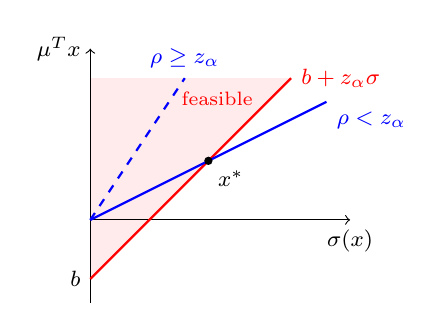
\begin{tikzpicture}[scale=0.75]
\fill[red!8] (0,-1) -- (3.4,2.4) -- (0,2.4) -- cycle;
\draw[->] (0,0) -- (4.4,0) node[below] {\footnotesize $\sigma(x)$};
\draw[->] (0,-1.4) -- (0,2.9) node[left] {\footnotesize $\mu^Tx$};
\draw[red, thick] (0,-1) -- (3.4,2.4) node[right] {\footnotesize $b + z_{\alpha}\sigma$};
\draw[blue, thick] (0,0) -- (4,2) node[below right] {\footnotesize $\rho < z_{\alpha}$};
\draw[blue, thick, dashed] (0,0) -- (1.6,2.4) node[above] {\footnotesize $\rho \geq z_{\alpha}$};
\fill (2,1) circle (2pt) node[below right] {\footnotesize $x^*$};
\node[left] at (0,-1) {\footnotesize $b$};
\node[red] at (2.15,2.05) {\scriptsize feasible};
\end{tikzpicture}
\end{column}
\end{columns}

\end{frame}

\begin{frame}
\frametitle{Generalization}

A more general form is
\begin{align*}
	\min_x \ & h(x) \\
	\text{s.t. } & P[ g_1(x, \bxi) \leq 0,\ldots, g_r(x, \bxi) \leq 0] \geq 1-\alpha \\
	& h_1(x) \leq 0,\ldots, h_m(x) \leq 0.
\end{align*}
Using $G(x, \bxi) = \max_{j=1,\dots,r} g_j(x, \bxi)$, the chance constraint can be expressed via the indicator of feasibility:
\[
\EE\left[ \mathbb{I}_{(-\infty, 0]} \left( G(x, \bxi) \right) \right] \geq 1-\alpha, \quad \text{where} \quad
\mathbb{I}_{(-\infty,0]}(t) =
\begin{cases}
	1 & \text{if } t \leq 0,\\
	0 & \text{if } t > 0,
\end{cases}
\]
or equivalently via the violation indicator $\mathbb{I}_{(0,\infty)}$:
\[
\EE\left[ \mathbb{I}_{(0,\infty)} \left( G(x, \bxi) \right) \right] \leq \alpha, \quad \text{where} \quad
\mathbb{I}_{(0,\infty)}(t) =
\begin{cases}
	1 & \text{if } t > 0,\\
	0 & \text{if } t \leq 0.
\end{cases}
\]

\end{frame}

\begin{frame}
\frametitle{Solution methods for the general case}

\begin{itemize}
\item	
Usually very hard.
\item
Use a bounding approximation or sample average approximation (SAA).
\item
We will discuss it in more detail when introducing Monte Carlo techniques.
\end{itemize}

\end{frame}

\begin{frame}
\frametitle{Probabilistic programming}

Source: András Prékopa (2003), ``Probabilistic Programming'', Chapter 5 in ``Stochastic Programming'', A. Ruszczy\'nski and A. Shapiro (editors), Elsevier.

\mbox{}

\begin{itemize}
	\item 
Sometimes we only want to maximize a probability.
\item
General form:
\begin{align*}
\max_x \ & P[ g_1(x, \bxi) \leq 0,\ldots, g_r(x, \bxi) \leq 0] \\
\text{s.t. } & h_1(x) \leq 0,\ldots, h_m(x) \leq 0.
\end{align*}
\end{itemize}

\end{frame}

\begin{frame}
\frametitle{Measures of violation}

\begin{itemize}
\item 
A chance constraint allows constraint violation with some probability.
\item
The violation can be large.
\item
It is often desirable to avoid too large violations.
\item
Can we penalize the violation?
\end{itemize}

\end{frame}

\begin{frame}
\frametitle{Value at Risk}

Source: \url{https://web.stanford.edu/class/ee364a/lectures/chance_constr.pdf}

\mbox{}

Value-at-risk of a loss $Z$ (large values are bad), at level $\eta \in (0,1)$:
\[
\text{VaR}(Z;\eta) = \inf \{ \gamma \mid P[Z \leq \gamma] \geq \eta \}
\]

\mbox{}

Therefore, the value-at-risk is simply the inverse of the cdf evaluated at $\eta$:
\[
\text{VaR}(Z;\eta) = F_Z^{-1}(\eta).
\]

\end{frame}

\begin{frame}
\frametitle{Conditional Value at Risk}

\[
\text{CVaR}(Z; \eta) = \inf_{\beta} \left( \beta + \frac{1}{1 - \eta} \EE \left[ (Z - \beta)_+ \right] \right).
\]

\smallskip

Assume that the distribution of $Z$ is continuous.

\smallskip

Solution $\beta^*$ obtained by solving
\[
0 = \frac{d}{d \beta} \left( \beta + \frac{1}{1 - \eta} \EE \left[ (Z - \beta)_+ \right] \right)
= 1 - \frac{1}{1 - \eta} P[ Z \geq \beta ],
\]
leading to
\[
P[ Z \geq \beta^* ] = 1 - \eta
\quad \Longleftrightarrow \quad P[ Z \leq \beta^* ] = \eta,
\]
satisfied by $\beta^* = \text{VaR}(Z; \eta)$, and only by it if $F_Z$ is strictly increasing.

\end{frame}

\begin{frame}
\frametitle{Expected shortfall}

Conditional tail expectation (or expected shortfall):
\begin{align*}
\EE[Z \mid Z \geq \beta^* ]
&= \EE[\beta^* + (Z - \beta^*) \mid Z \geq \beta^*] \\
&= \beta^* + \frac{\EE\left[(Z - \beta^*)_+\right]}{P[Z \geq \beta^*]} \\
&= \text{CVaR}(Z; \eta)
\end{align*}

\begin{itemize}
	\item Can be added to the objective.
	\item Can be used as a constraint: \textit{conditional expectation constraint}
	\[
	\EE[Z \mid Z \geq \beta^*] \leq d.
	\]
\end{itemize}

\end{frame}

\begin{frame}
\frametitle{CVaR and chance constraints}

In the continuous case, $\text{CVaR}(Z;\eta)$ is the mean of $Z$ beyond $\text{VaR}(Z;\eta)$, hence $\text{VaR}(Z;\eta) \leq \text{CVaR}(Z;\eta)$ (true in general).
With $Z = G(x,\bxi)$ and $\eta = 1-\alpha$:
\[
\text{CVaR}(G(x,\bxi); 1-\alpha) \leq 0
\ \Longrightarrow\
\text{VaR}(G(x,\bxi); 1-\alpha) \leq 0
\ \Longleftrightarrow\
P[G(x,\bxi) \leq 0] \geq 1-\alpha.
\]
By definition of the CVaR, the left-hand constraint holds if and only if, for some $\beta \in \RR$,
\[
\beta + \frac{1}{\alpha} \EE\left[ (G(x,\bxi) - \beta)_+ \right] \leq 0,
\]
{\red a convex constraint in $(x, \beta)$} when $G(\cdot,\xi)$ is convex: a conservative convex approximation of the chance constraint.
With finitely many scenarios and affine $g_j$, it is a set of linear constraints, with one auxiliary variable per scenario.

\smallskip

{\footnotesize (Rockafellar and Uryasev, 2000; Nemirovski and Shapiro, 2006)}

\end{frame}

\begin{frame}
\frametitle{Integrated chance constraints}

\begin{itemize}
\item 
Consider the stochastic constraints
\[
g_i(x, \bxi) \leq 0, \quad i = 1,\ldots, r.
\]
\item
Integrated chance constraint:
\[
\EE \left[ \max_{i=1,\ldots,r} (g_i(x,\bxi))_+ \right] \leq d.
\]
\item
Unlike a chance constraint, it defines a {\red convex set for any distribution} of $\bxi$, as soon as the $g_i$ are convex in $x$.
With a finite discrete distribution and affine $g_i$, this set is a polyhedron: the constraint can be handled by linear programming.
\end{itemize}

\smallskip

{\footnotesize For more details, see Chapter 6 (Section 6.3 for joint constraints), Willem K. Klein Haneveld, Maarten H. van der Vlerk, Ward Romeijnders (2020), ``Stochastic Programming - Modeling Decision Problems Under Uncertainty'', Springer.\par}
\end{frame}

%% More to read in Prékopa, starting from Section 2.

\end{document}